\documentclass[handout]{ximera}
%handout:  for handout version with no solutions or instructor notes
%handout,instructornotes:  for instructor version with just problems and notes, no solutions
%noinstructornotes:  shows only problem and solutions

%% handout
%% space
%% newpage
%% numbers
%% nooutcomes

%I added the commands here so that I would't have to keep looking them up
%\newcommand{\RR}{\mathbb R}
%\renewcommand{\d}{\,d}
%\newcommand{\dd}[2][]{\frac{d #1}{d #2}}
%\renewcommand{\l}{\ell}
%\newcommand{\ddx}{\frac{d}{dx}}
%\everymath{\displaystyle}
%\newcommand{\dfn}{\textbf}
%\newcommand{\eval}[1]{\bigg[ #1 \bigg]}

%\begin{image}
%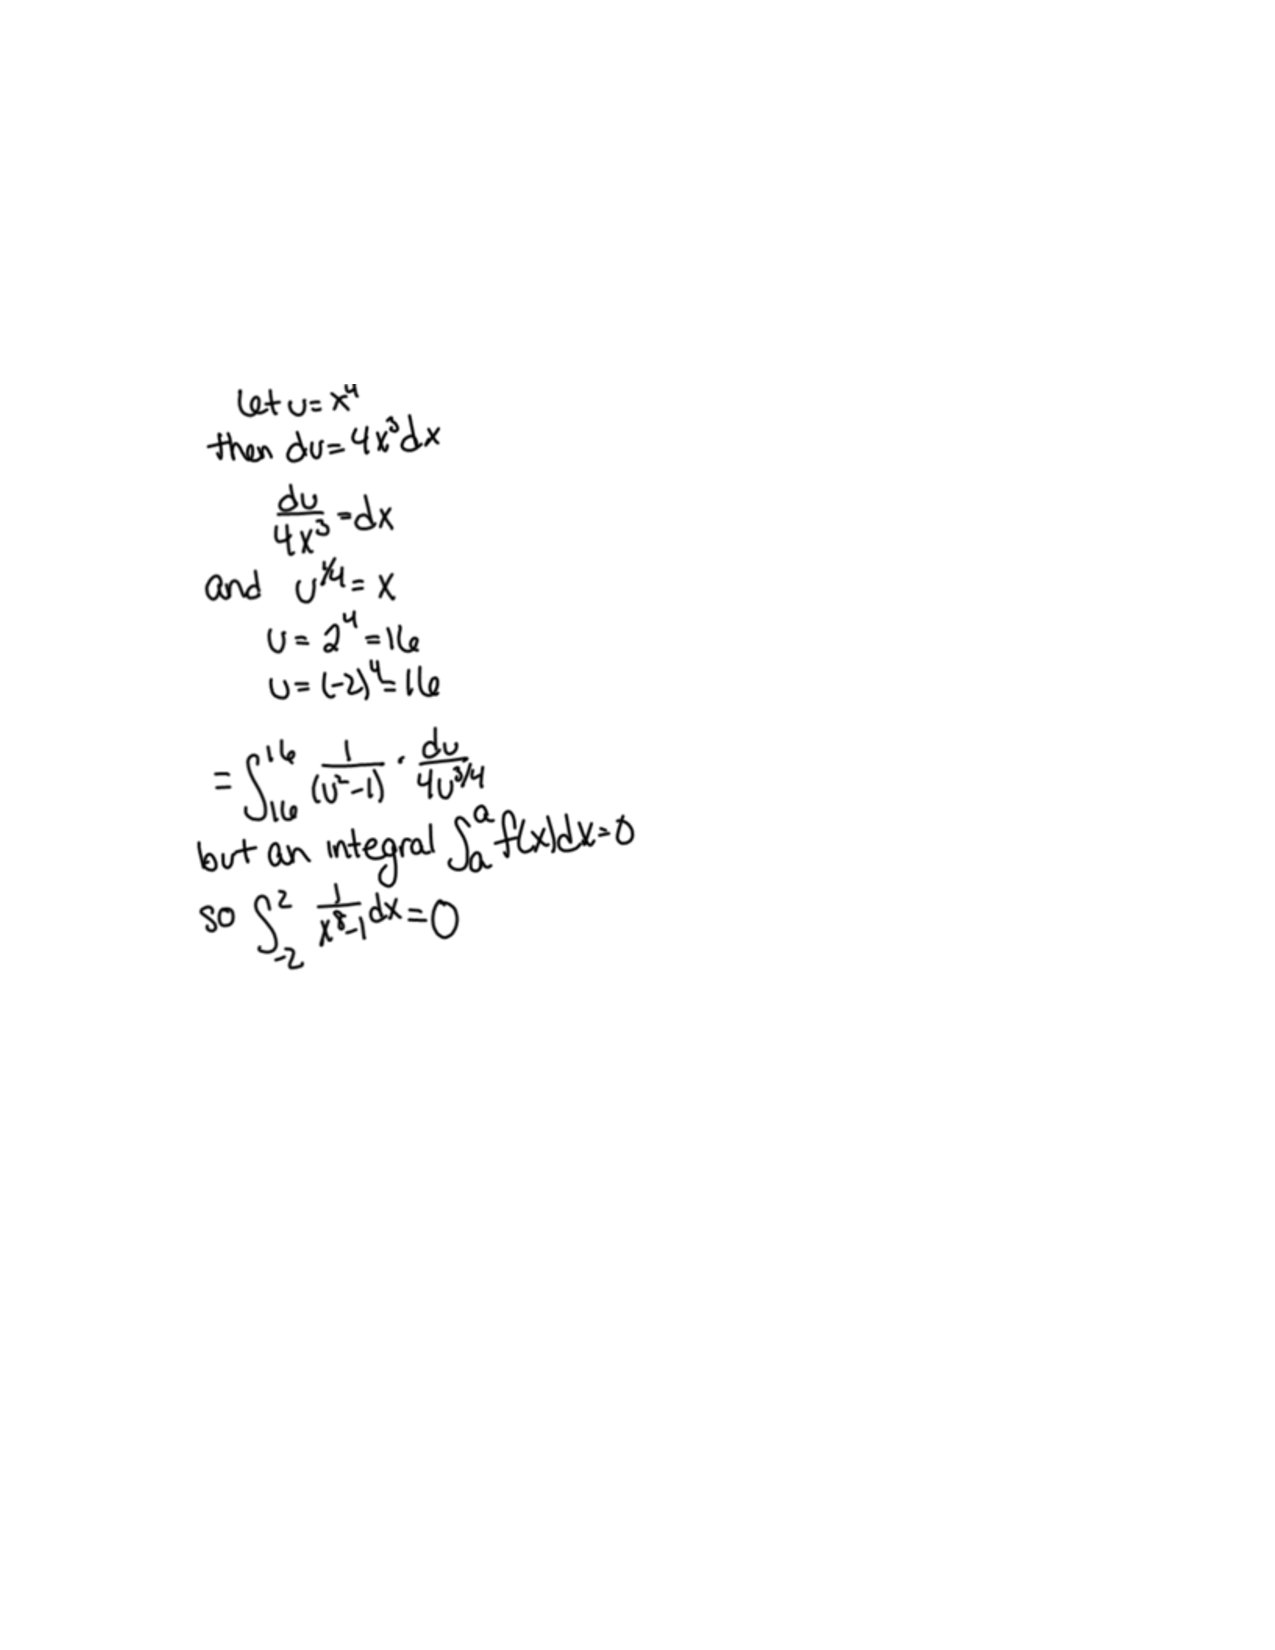
\includegraphics[trim= 170 420 250 180]{Figure1.pdf}
%\end{image}

%add a ``.'' below when used in a specific directory.
\newcommand{\RR}{\mathbb R}
\renewcommand{\d}{\,d}
\newcommand{\dd}[2][]{\frac{d #1}{d #2}}
\renewcommand{\l}{\ell}
\newcommand{\ddx}{\frac{d}{dx}}
\newcommand{\dfn}{\textbf}
\newcommand{\eval}[1]{\bigg[ #1 \bigg]}

\usepackage{multicol}

\renewenvironment{freeResponse}{
\ifhandout\setbox0\vbox\bgroup\else
\begin{trivlist}\item[\hskip \labelsep\bfseries Solution:\hspace{2ex}]
\fi}
{\ifhandout\egroup\else
\end{trivlist}
\fi} %% we can turn off input when making a master document

\title{Sections 12.2: Vectors in Three Dimensions}  

\begin{document}
\begin{abstract}		\end{abstract}
\maketitle








\section{Group work:}


%problem 5
\begin{problem}
Solve the following problems:
	\begin{enumerate}
	\item  Which of the points $(6,2,3)$, $(-5,-1,4)$, and $(0,3,8)$ is closest to the $xz$-plane?  
	Which point lies on the $yz$-plane?
	
	\item  Write an equation of the circle of radius $2$ centered at $(-3,4,1)$ that lies in a plane parallel to the $xy$-plane.
	
	\item  Describe the sphere $x^2 + y^2 + z^2 + 6x - 14y - 2z = 5$ (ie, find its center and radius).
	
	\item  Find a vector whose magnitude is $311$ and is in the same direction as the vector $\langle 3,-6,7 \rangle$.
	\end{enumerate}
	
	\begin{freeResponse}
	\begin{enumerate}
	\item  The $xz$-plane has equation $y=0$.  
	The distance from a point $(a,b,c)$ to $y=0$ is just $|b|$.  
	So
		\begin{align*}
		&(6,2,3) \text{ has distance }2  \\
		&(-5,-1,4) \text{ has distance }1  \\
		&(0,3,8) \text{ has distance }3
		\end{align*}
	Therefore, the point $(-5,-1,4)$ is closest to the $xz$-plane.  
	
	The $yz$-plane is $x=0$, and so the point $(0,3,8)$ is on the $yz$-plane.
	
	
	
	\item  A plane parallel to the $xy$-plane has equation $z = \#$.  
	We are looking for such a plane containing the point $(-3,4,1)$, and so the plane is $z=1$.  
	Therefore, the equation is
		\[
		\boxed{ (x+3)^2 + (y-4)^2 = 4 \;, \; z = 1.   }
		\]
		
		
	
%	\item  We complete the square with respect to all three variables.
%		\begin{align*}
%		x^2 + y^2 + z^2 + 6x - 14y - 2z &= 5  \\
%		(x^2 + 6y + 9) + (y^2 - 14y + 49) + (z^2 - 2z + 1) &= 5 + 9 + 49 + 1  \\
%		(x+3)^2 + (y-7)^2 + (z-1)^2 &= 64.
%		\end{align*}
%	So, the center of the sphere is $(-3,7,1)$ and its radius is $8$.
%	
	
	
	\item  Let $\vec{v} = \langle 3,-6,7 \rangle$.  
	Then
		\begin{align*}
		| \vec{v} | &= \sqrt{3^2 + (-6)^2 + 7^2}  \\
		&= \sqrt{9 + 36 + 49}  \\
		&= \sqrt{94}.
		\end{align*}
	So a unit vector in the same direction as $\vec{v}$ is
		\[
		\frac{1}{\sqrt{94}} \langle 3,-6,7 \rangle
		\]
	and therefore a vector with magnitude $311$ in the same direction as $v$ is
		\[
		\boxed{\frac{311}{\sqrt{94}} \langle 3,-6,7 \rangle}
		\]
	
	\end{enumerate}
	\end{freeResponse}
	
\end{problem}

\begin{instructorNotes}

\end{instructorNotes}











	
	
	
	
	
	
	
	
	

	










								
				
				
	














\end{document} 


















